\documentclass[conference]{IEEEtran}
%+++++++++++++++++++++++++++++++++++++++++++
% Added to commands
\input epsf
\usepackage{graphicx}
\usepackage [french]{babel}
\usepackage [utf8]{inputenc}
\usepackage [T1] {fontenc}
\usepackage{array}
\usepackage{subfigure} % Pour créer des sous-figures (option ancienne)
\usepackage{float}
%+++++++++++++++++++++++++++++++++++++++++++
% correct bad hyphenation here
\hyphenation{op-tical net-works semi-conduc-tor IEEEtran}
\begin{document}

%+++++++++++++++++++++++++++++++++++++++++++
\title{\LARGE Etude de l'influence du couple (diamètre, profondeur) sur la finesse d'un kite
\vskip10pt

\small 2024 - Romain LAMBERT
}
%+++++++++++++++++++++++++++++++++++++++++++
% make the title area
\maketitle

\begin{abstract}Ce bureau d'étude a pour sujet l'étude de l'influence du \textbf{diamètre} (diameter) et de la \textbf{cambrure} (depth) sur la finesse d'un kite. L'objectif final étant de déterminer un couple (t,k) = (diameter, depth) qui serve de référence pour le dimensionnement des kites. Aussi, cette étude permet d'évaluer la sensibilité de la \textbf{VSM} sous la théorie 2D de la \textbf{regression de Breukels} à ces deux paramètres.
\end{abstract}
\IEEEoverridecommandlockouts

\IEEEpeerreviewmaketitle
\section{La théorie}

\subsection{\textbf{Regresion de Breukels : théorie 2D}} 

Si la VSM permet d'étudier l'aérodynamique 3D d'un kite, elle requiert le calcul des coefficients 2D de chaque section($C_L$, $C_D$, $C_M$). Afin de limiter le coût de calcul et de se baser sur des polaires adaptées à des profils "non conventionnels", la VSM utilise une \underline{formule de regression de Breukels}. 
Cette formule est issue de résultats obtenus sur des profils typiques de kites à boudin, et ne \underline{dépend que du diamètre du boudin et de la cambrure du profil}. \\


\begin{center}
    \begin{equation}
        C_L = \lambda_5  \alpha^3 +\lambda_6  \alpha^2 + \lambda_7  \alpha + \lambda_8
        \label{eq:Cl_breukels}
    \end{equation}
\end{center}
avec :
\begin{center}
    \begin{equation}
        \lambda_i = S_x  k + S_y
        \label{eq:lamba_breukels}
    \end{equation}
\end{center}
et :
\begin{center}
    \begin{equation}
        S_i = C_x  t^2 + C_y  t + C_z
        \label{eq:S_breukels}
    \end{equation}
\end{center}
où les 23 coéfficients $C_x$ sont prédéterminés, et (t,k) est le couple (diamètre, cambrure) définit tel que :
\begin{center}
    \begin{equation}
        t = \frac{Diamètre(BA)}{Corde} ; k = \frac{max(CoordonéesExtrados)}{Corde}
        \label{eq:tk_breukels}
    \end{equation}
\end{center}

Ainsi, l'obtention ds coéfficients 2D permet ensuite à la VSM d'ajouter l'indluence des effets 3D (loi de corde, d'envergure, de voute...) sur les coefficients aérodynamiques d'un kite

\begin{figure}[H]
    \centering
    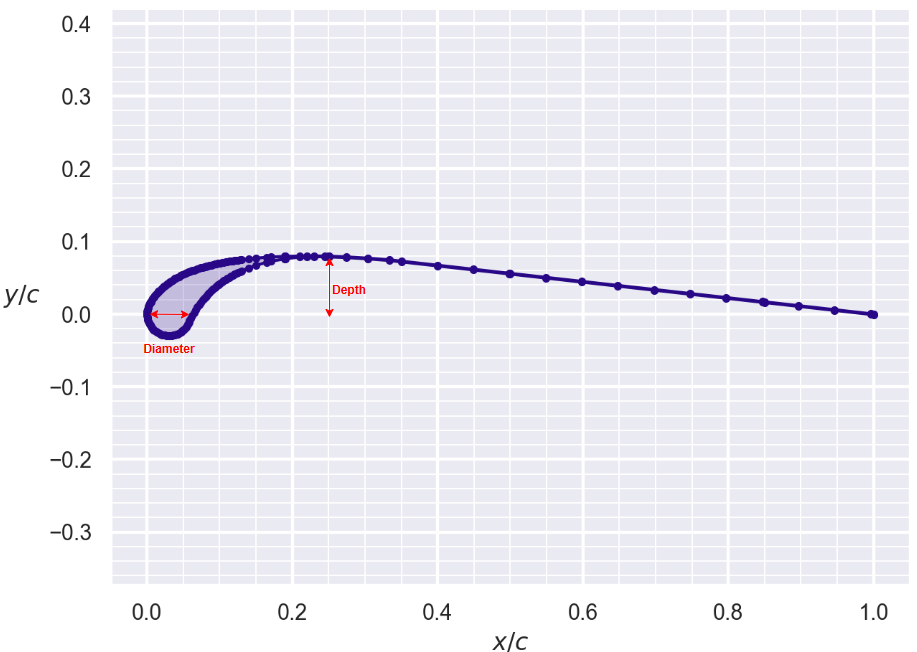
\includegraphics[width=0.5\textwidth]{Pics/airfoil.png}  
    \caption{Profil central d'une SK50-VG avec identification du diamètre et de la cambrure tel que utilisés par la VSM.}
    \label{fig:airfoil}
\end{figure}

%%%%%%%%%%%%%%%%%%%%%%%%%%%%%%%%%%%%%%%%%%%%%%%%%%%%%%%%%%%%%%%%%%%%%%%%%
\IEEEpeerreviewmaketitle
\section{Le Code }

\subsection{Le cas d'étude - 2D} 

On étudie dans un premier temps La fonction de Breukels pour en chercher les optimum. On utilise pour ce faire un code d'optimsiation fournit par la bibliothèque \textbf{aerosandbox} et on se place dans le cas d'optimisation suivant: 
\begin{itemize}
    \item Maximum de $\sum_{\alpha = 0}^{20}\frac{C_L(\alpha)}{C_D(\alpha)} Gaussienne(alpha, center, sigma) $
\end{itemize}

    où $Gaussienne(\alpha, center, \sigma) = e^{-\frac{(center - \alpha)^2}{2\sigma^2}}$ est une Gaussienne permettant d'obtenir une moyenne pondérée. 

\underline{Les résultats sont présentés dans la partie suivante.}
\begin{figure}[H]
    \centering
    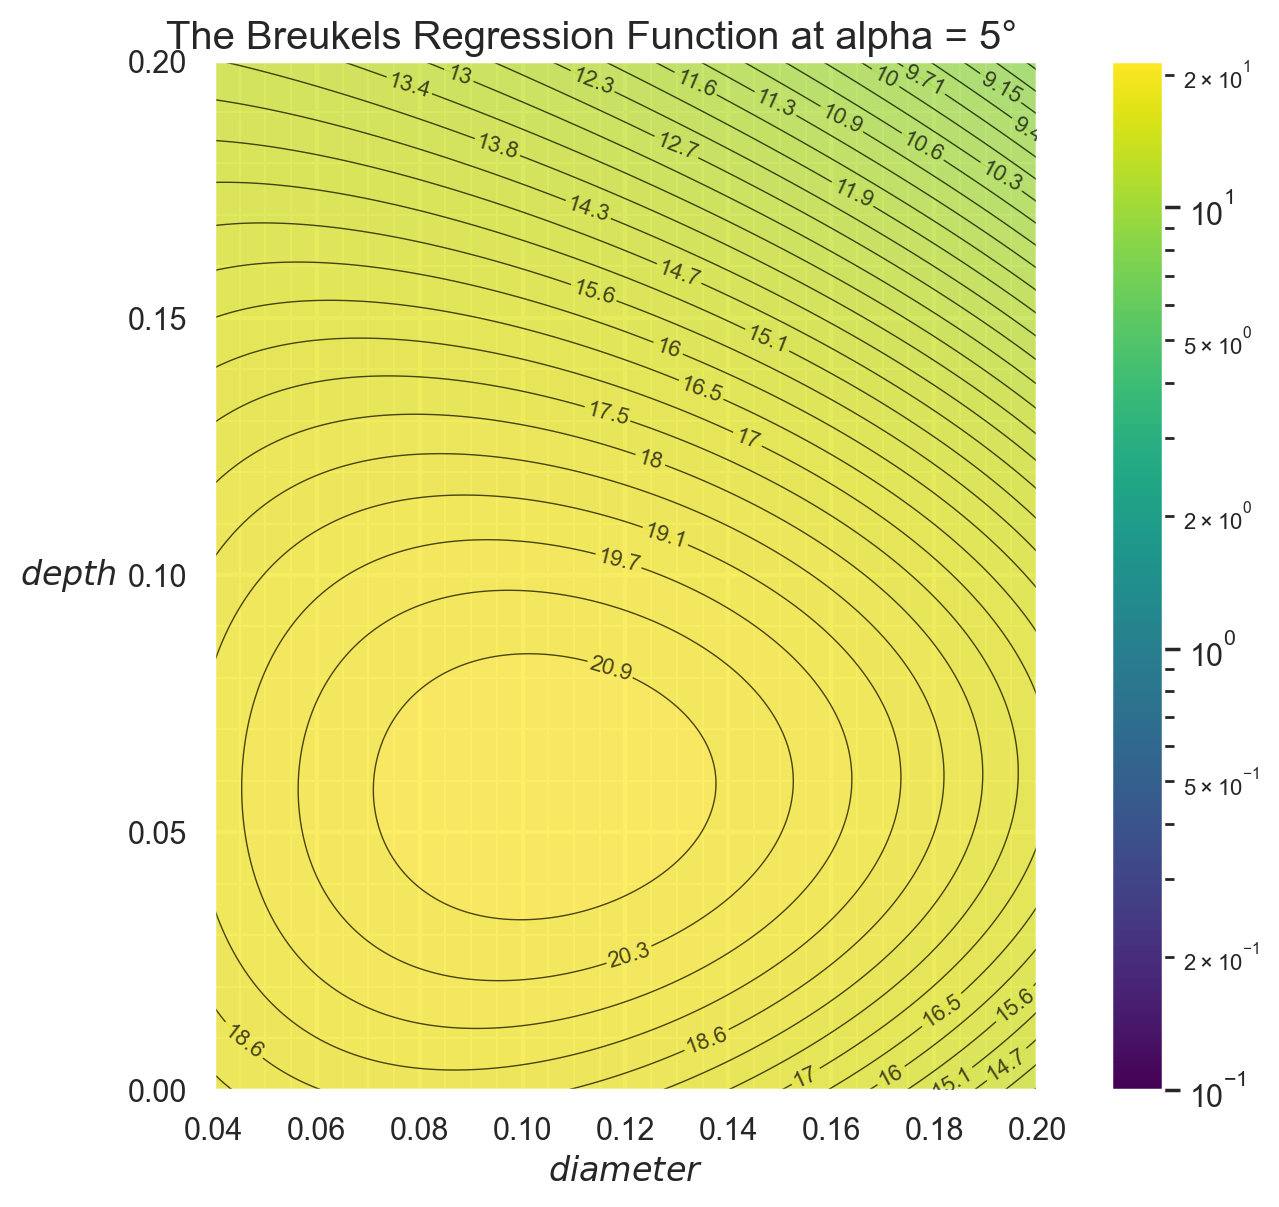
\includegraphics[width=0.5\textwidth]{Pics/breukels.png}  
    \caption{Tracer de $\frac{C_L}{C_D}$ par Régression de Breukels à $\alpha$=5°}
    \label{fig:breukels}
\end{figure}


\subsection{Le cas d'étude - 3D} 

\textbf{L'étude est réalisée à 50 knots}.\\
On se place dans le cas d'étude d'un SK50-VG dont on fait varier le \textbf{diamètre t entre -0.02 et +0.1 et la cambrure k entre -0.1 et 0.1}. \\
    
    On ajoute sur chaque rib les limites suivantes :
    \begin{itemize}
        \item \textbf{le diamètre ne peut pas être inférieur à 0.04}
        \item \textbf{la cambrure ne peut pas être inférieure au demi-diamètre}
    \end{itemize}

    Ainsi, les résultats sont à nuancer : \textbf{une aile avec un certain delta de t ou de k ne veut pas dire que toutes les sections ont été modifiées de ce delta; seules les sections respectant ces critères de minimum énoncés précédemment le sont.}

La loi d'évolution de t et k sur une VG est initialement:  
\begin{itemize}
    \item t : [0.07 0.067 0.065 0.063 0.061 0.06 0.06  0.06 0.06 0.06  0.06  0.06 0.06 0.06  0.06 0.061 0.063 0.065 0.067 0.07]
    \item k : [0.034 0.05 0.0645 0.0686 0.072 0.075 0.08 0.08 0.08 0.08      0.08 0.08 0.08 0.08 0.075 0.072 0.0686 0.0645 0.05 0.034]
\end{itemize}

    A nouveau, on cherche l'optimum dans le problème d'optimisation suivants:
    \begin{itemize}
        \item Maximum de $\sum_{\alpha = 0}^{21}\frac{C_L(\alpha)}{C_D(\alpha)} Gaussienne(alpha, center, sigma) $
    \end{itemize}
    \underline{Les résultats sont présentés dans la partie suivante.}

\begin{figure}[H]
    \centering
    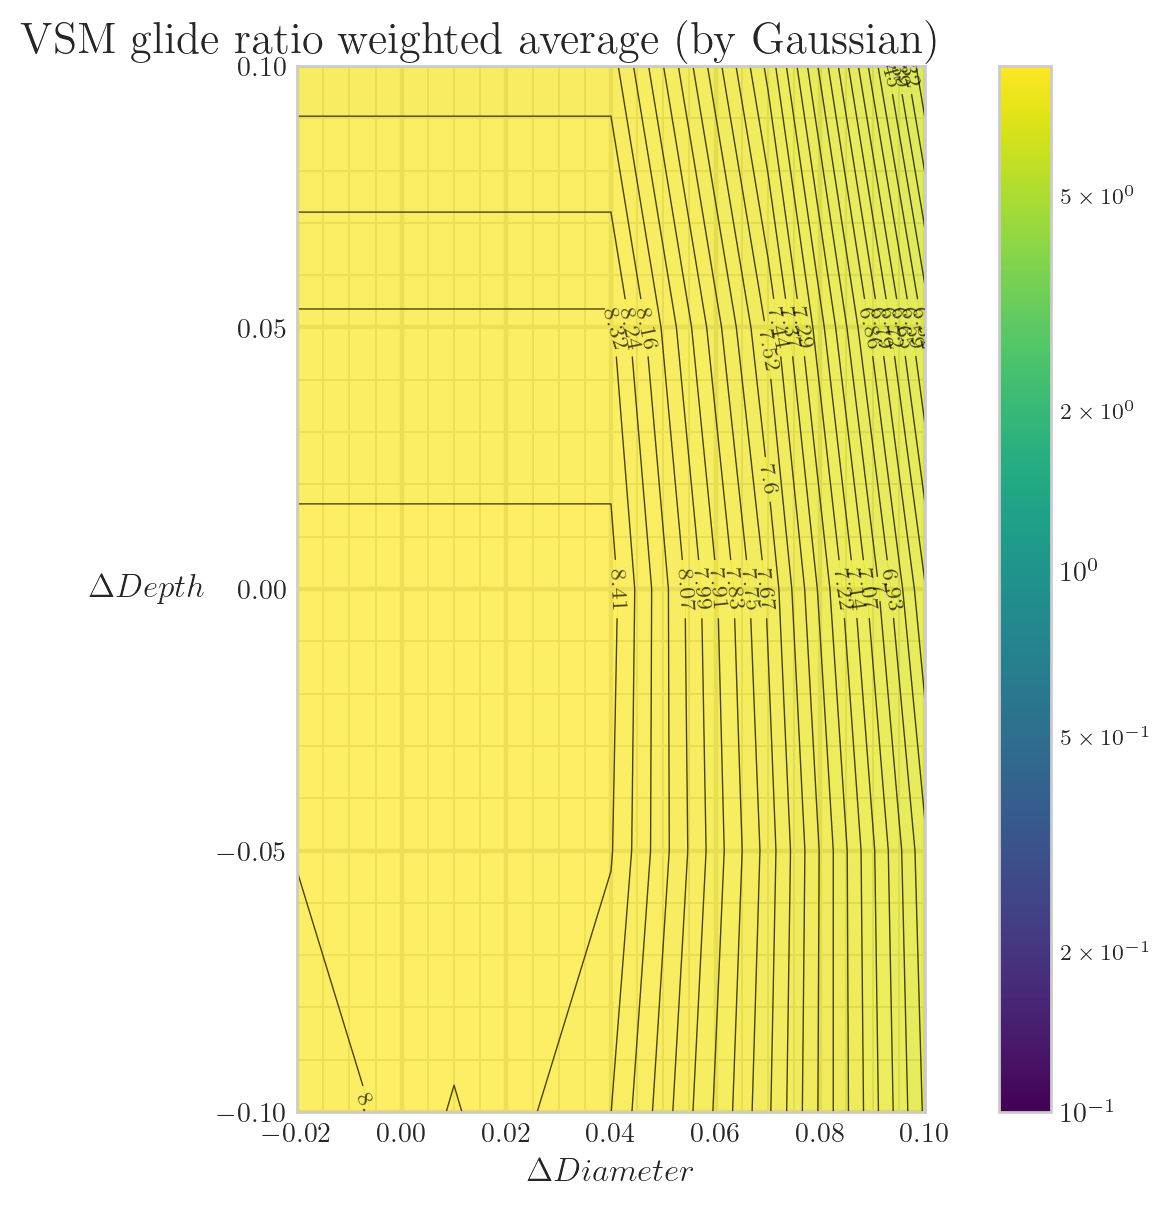
\includegraphics[width=0.5\textwidth]{Pics/vsm.png}  
    \caption{Tracer de $\frac{C_L}{C_D}$ par VSM en faisant varier (t,k)}
    \label{fig:vsm}
\end{figure}


%%%%%%%%%%%%%%%%%%%%%%%%%%%%%%%%%%%%%%%%%%%%%%%%%%%%%%%%%%%%%%%%%%%%%%%%%
\IEEEpeerreviewmaketitle
\section{Les Résultats}

\subsection{2D - résultats par alpha}

\begin{figure}[h!]
    \centering
    \begin{minipage}[b]{0.45\textwidth}
        \centering
        \begin{tabular}{|c|c|c|}
            \hline
            \textbf{$\alpha$} & \textbf{$diamètre_{opti}$} & \textbf{$cambrure_{opti}$}\\
            \hline
            0 & 0.040 & 0.20 \\
            1 & 0.091 & 0.00 \\
            2 & 0.098 & 0.00 \\
            3 & 0.10 & 0.01  \\
            4 & 0.10 & 0.04  \\
            5 & 0.10 & 0.06  \\
            6 & 0.10 & 0.068  \\
            7 & 0.095 & 0.074 \\
            8 & 0.089 & 0.078 \\
            9 & 0.079 & 0.082 \\
            10 & 0.061 & 0.086 \\
            11 & 0.040 & 0.093 \\
            12 & 0.040 & 0.103 \\
            13 & 0.040 & 0.105 \\
            14 & 0.040 & 0.107 \\
            15 & 0.040 & 0.109 \\
            16 & 0.040 & 0.111 \\
            17 & 0.040 & 0.113 \\
            18 & 0.040 & 0.115 \\
            19 & 0.040 & 0.118 \\
            20 & 0.040 & 0.121 \\
            \hline
        \end{tabular}
        \caption{Valeurs optimales pour chaque alpha}
        \label{fig:table}
    \end{minipage}
    \hfill % Séparation entre les deux blocs
    % Minipage pour le graphique à droite
    \begin{minipage}[b]{0.45\textwidth}
        \centering
        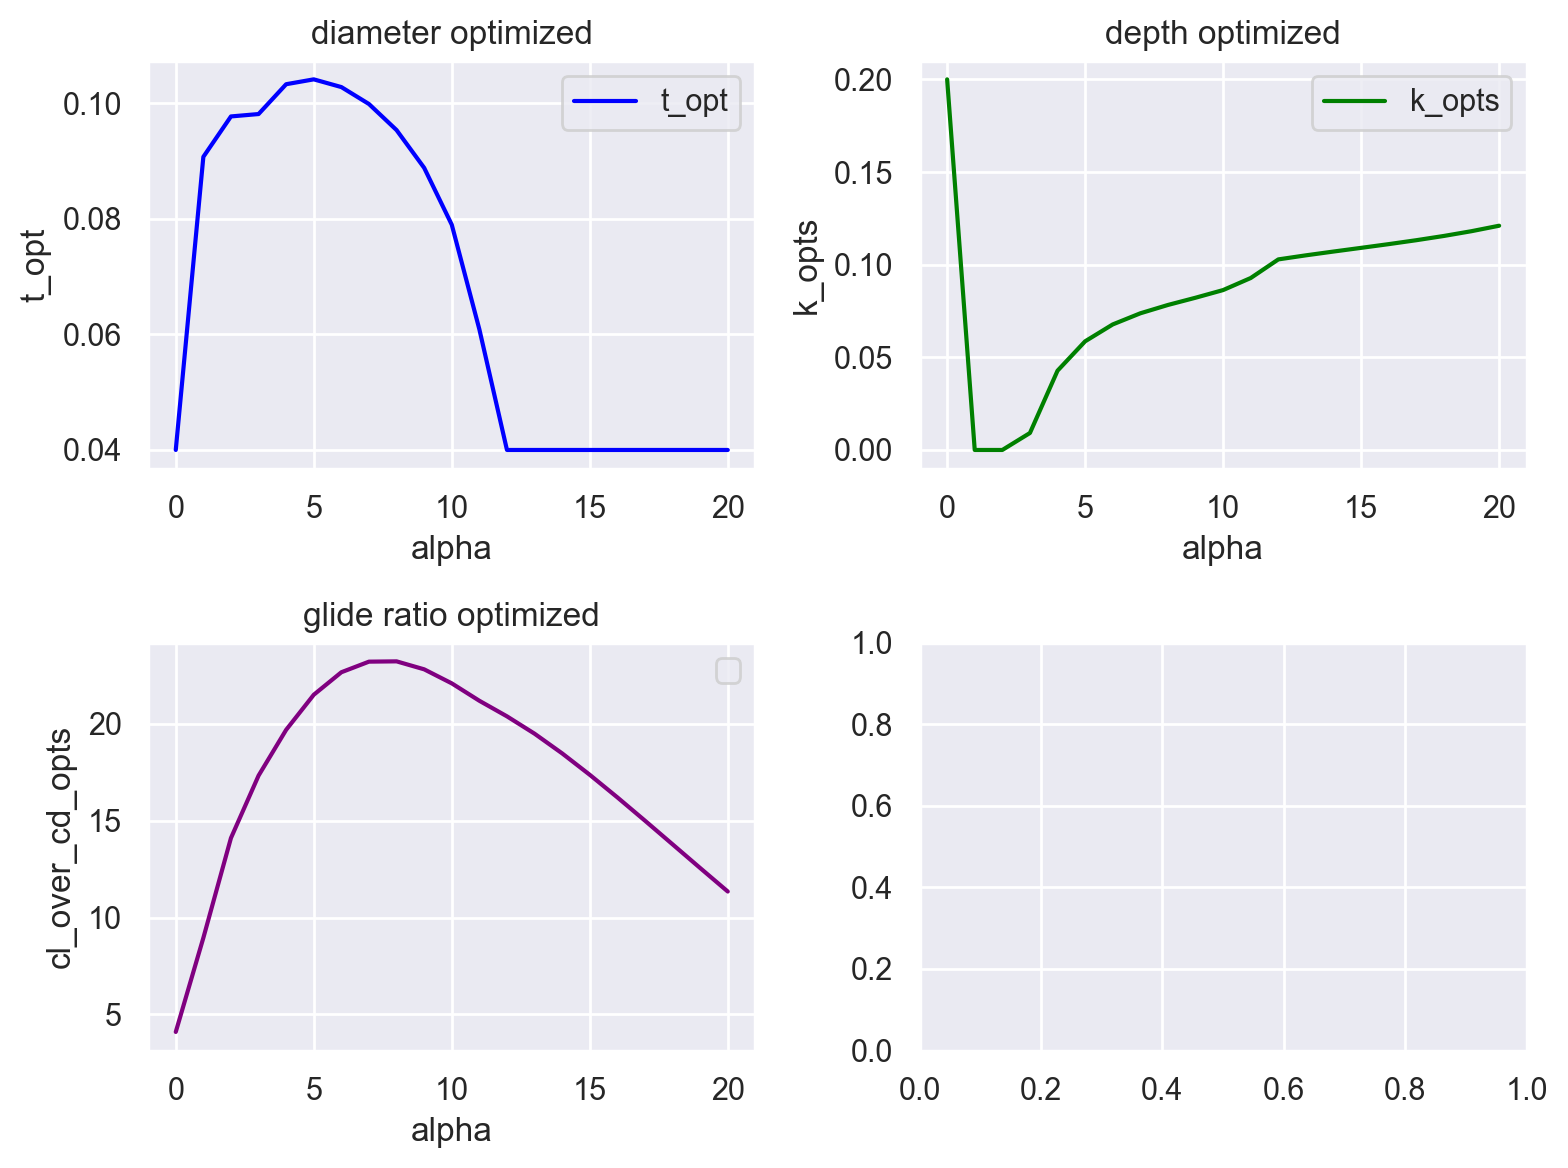
\includegraphics[width=\textwidth]{Pics/résultats pas alpha 2D.png}
        \caption{Tracer de t et k optimaux pour chaque alpha}
        \label{fig:graph}
    \end{minipage}
    \caption{Résultats 2D optimaux (finesse) de diamètre et cambrure par alpha}
    \label{fig:opti alpha 2d}
\end{figure}

\textbf{On observe que pour les grands angles le diamètre optimal tend à être le plus petit possible. La cambrure optimale augmente avec $\alpha$. Les résultats sont cohérents en ordre de grandeur}


\subsection{2D - résultats moyennes pondérées par Gaussienne}

\begin{figure}[h!]
    \centering
    \subfigure[diamètre selon les paramètres de la Gaussienne]{
        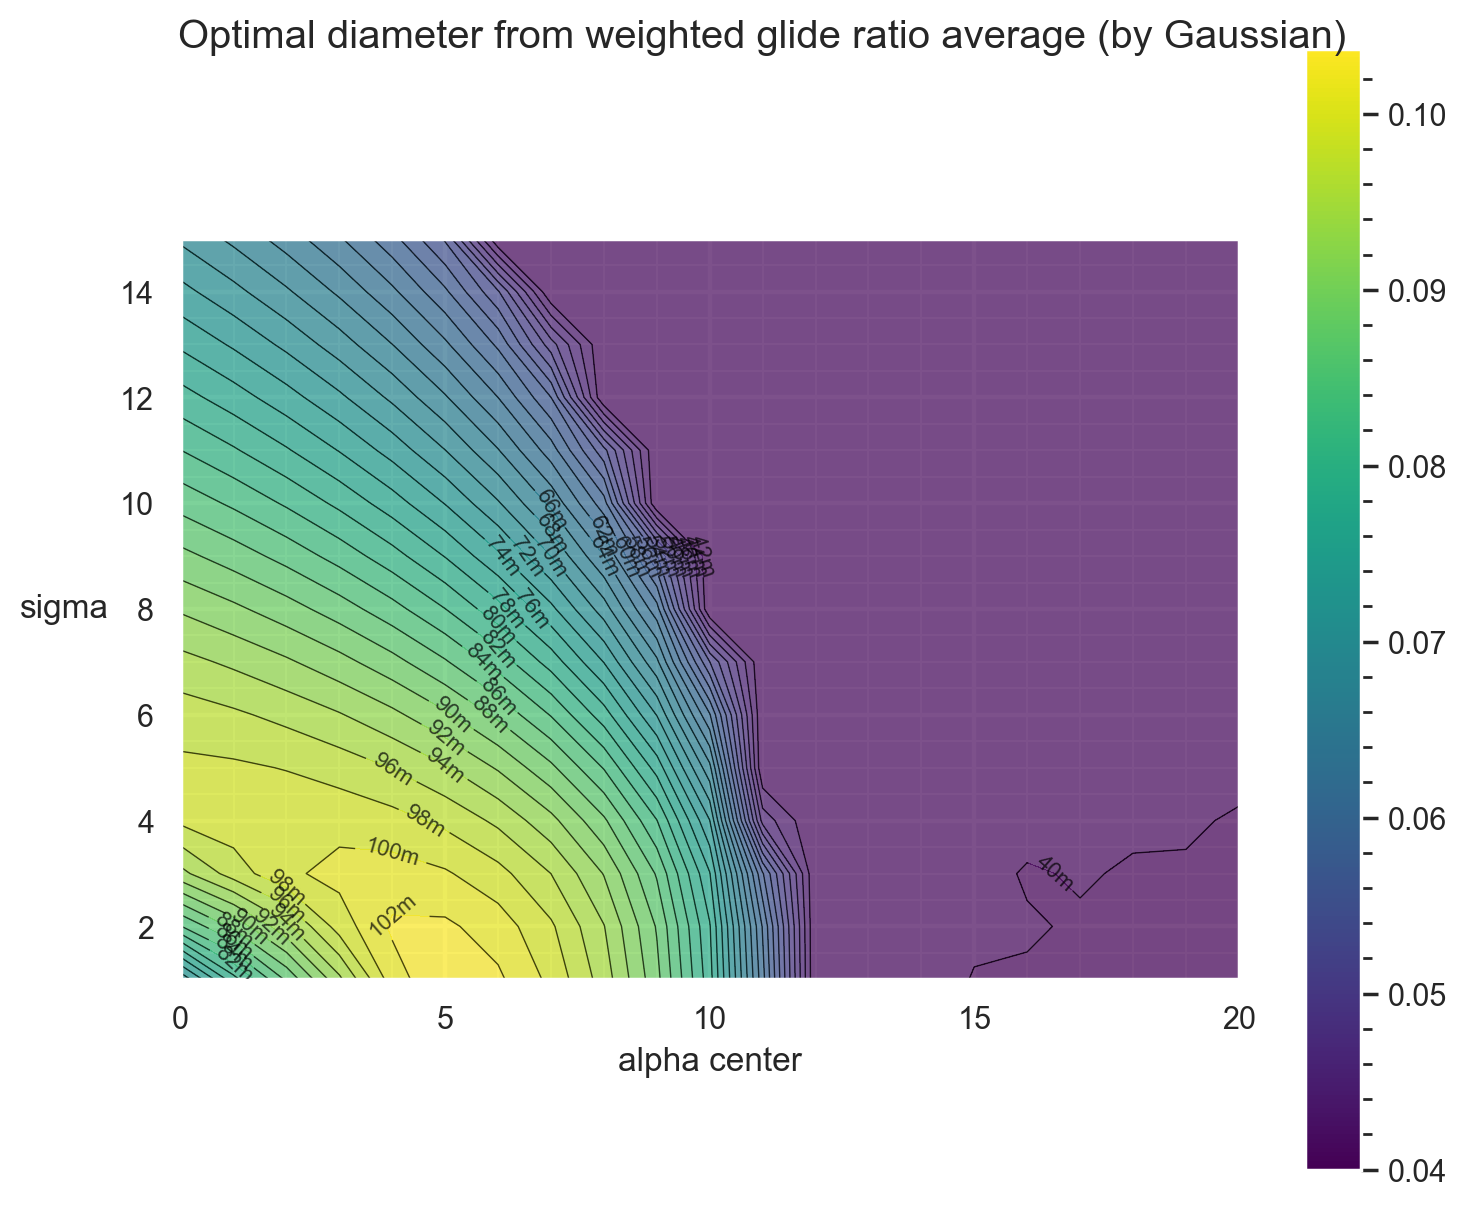
\includegraphics[width=0.45\textwidth]{Pics/diametre gaussian 2d.png}
        \label{fig:diametre gaussien 2d}
    }
    \hfill 
    \subfigure[cambrure selon les paramètres de la Gaussienne]{
        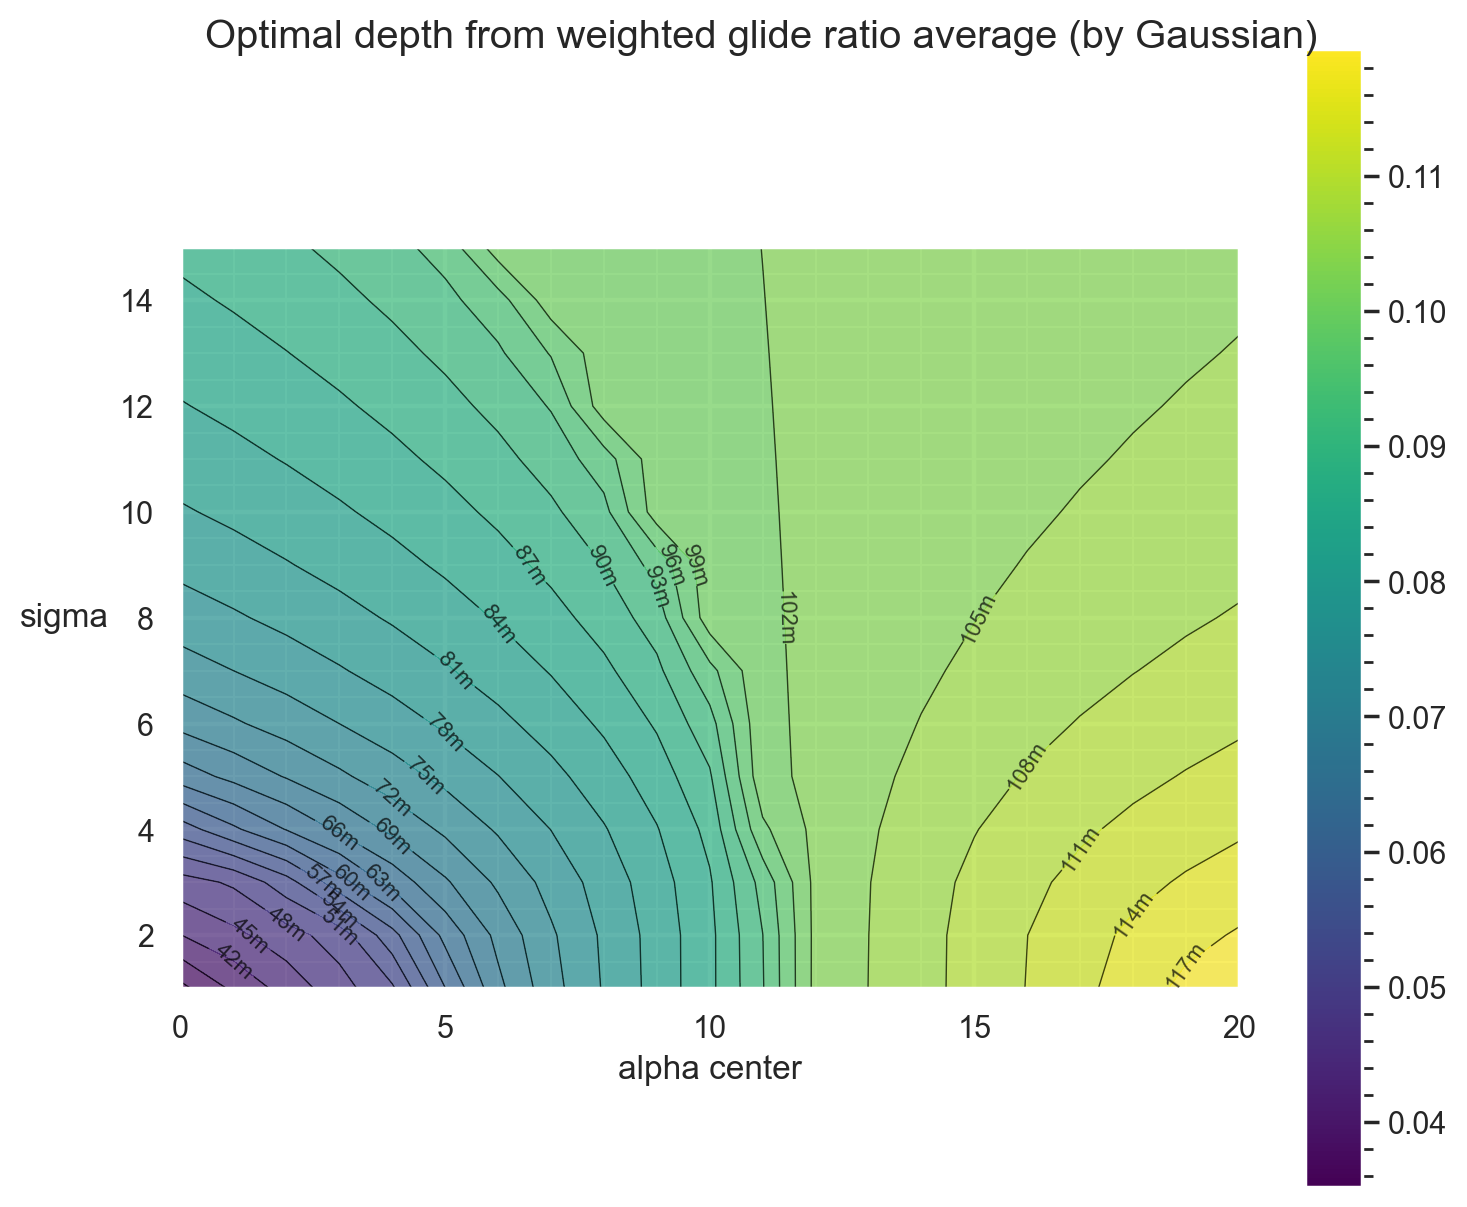
\includegraphics[width=0.45\textwidth]{Pics/depth gaussian 2d.png}
        \label{fig:cambrure gaussien 2d}
    }
    \caption{Sensibilté des résultats 2d en fonction de l'écart-type $\sigma$ et de la valeurs centrale $\alpha_{center}$ de la Gaussienne}
    \label{fig:gaussian sensibility 2d}
\end{figure}

\textbf{Pour $\sigma$ proche de zéro (écart-type "très petit"), les résultats convergent vers ceux de la partie précédente. }\\

\textbf{Le diamètre optimal} augmente avec $\alpha_{center}$ (jusqu'à environ 5°) puis diminue avec $\alpha_{center}$ pour des $\sigma$ inférieurs à 4. Augmenter $\sigma$ (i.e. "prendre davantage d'angles en considération") tend à diminuer le diamètre pour $\alpha_{center}$ plus grand que 5. Le diamètre optimal sature à sa valeurs minimale au delà de 12°. \\

\textbf{La cambrure optimale} augmente avec $\alpha$. Elle augmente avec $\sigma$ pour alpha inférieur à 12° et diminue avec $\sigma$ pour alpha plus grand.

\subsection{3D - résultats par alpha}

Le tableau suivant présente les résultats obtenu avec la VSM (3D). Les nombres de ribs saturés en diamètre/cambrure sont, pour chaque alpha, les nombre de ribs qui ne pouvaient pas atteindre la valeurs objective (Valeurs initiale + delta) et qui donc sont "saturés" à la valeurs minimal ( $\frac{Diamètre}{2}$ pour la cambrure et 0.04 pour le diamètre).\\

A noter que les ribs initialement à faible diamètre (relatif) sont ceux du bord d'attaque, et que les profils les moins cambré sont aux tips; en témoigne les valeurs initiales de t et k présentés en II.B..

\begin{figure}[H]
    \centering
    \begin{minipage}[b]{0.45\textwidth}
        \centering
        \begin{tabular}{|c|c|c|c|c|}
            \hline
            \textbf{$\alpha$} & \textbf{\parbox{1.5cm}{\centering $\delta$diamètre}} & \textbf{\parbox{1.5cm}{\centering nombre ribs saturés en diamètre}} & \textbf{\parbox{1.5cm}{\centering $\delta$cambrure}} & \textbf{\parbox{1.5cm}{\centering nombre ribs saturés en cambrure}}\\
            \hline
            0 & -0.02 & 10 & -0.1 & 20\\
            1 & -0.007 & 0 & -0.1 & 20\\
            2 & -0.007 & 0 & -0.1 & 20\\
            3 & -0.007 & 0 & -0.1 & 20 \\
            4 & -0.007 & 0 & -0.1 & 20 \\
            5 & -0.007 & 0 & -0.1 & 20 \\
            6 & -0.007 & 0 & -0.1 & 20  \\
            7 & -0.007 & 0 & -0.1 & 20 \\
            8 & -0.02 & 0 & -0.1 & 20 \\
            9 & -0.02 & 0 & -0.1 & 20 \\
            10 & -0.02 & 0 & -0.1 & 20 \\
            11 & 0.033 & 0 & -0.033 & 12 \\
            12 & 0.033 & 0 & -0.033 & 12 \\
            13 & 0.033 & 0 & -0.1 & 4 \\
            14 & 0.02 & 0 & -0.1 & 4 \\
            15 & 0.02 & 0 & -0.1 & 4 \\
            16 & 0.02 & 0 & -0.1 & 4 \\
            17 & 0.02 & 0 & -0.1 & 4 \\
            18 & -0.007 & 0 & 0.1 & 0 \\
            19 & -0.007 & 0 & 0.1 & 0 \\
            20 & -0.007 & 0 & 0.1 & 0 \\
            \hline
        \end{tabular}
        \caption{Valeurs optimales pour chaque alpha}
        \label{fig:table}
    \end{minipage}
    \hfill 
    \begin{minipage}[b]{0.45\textwidth}
        \centering
        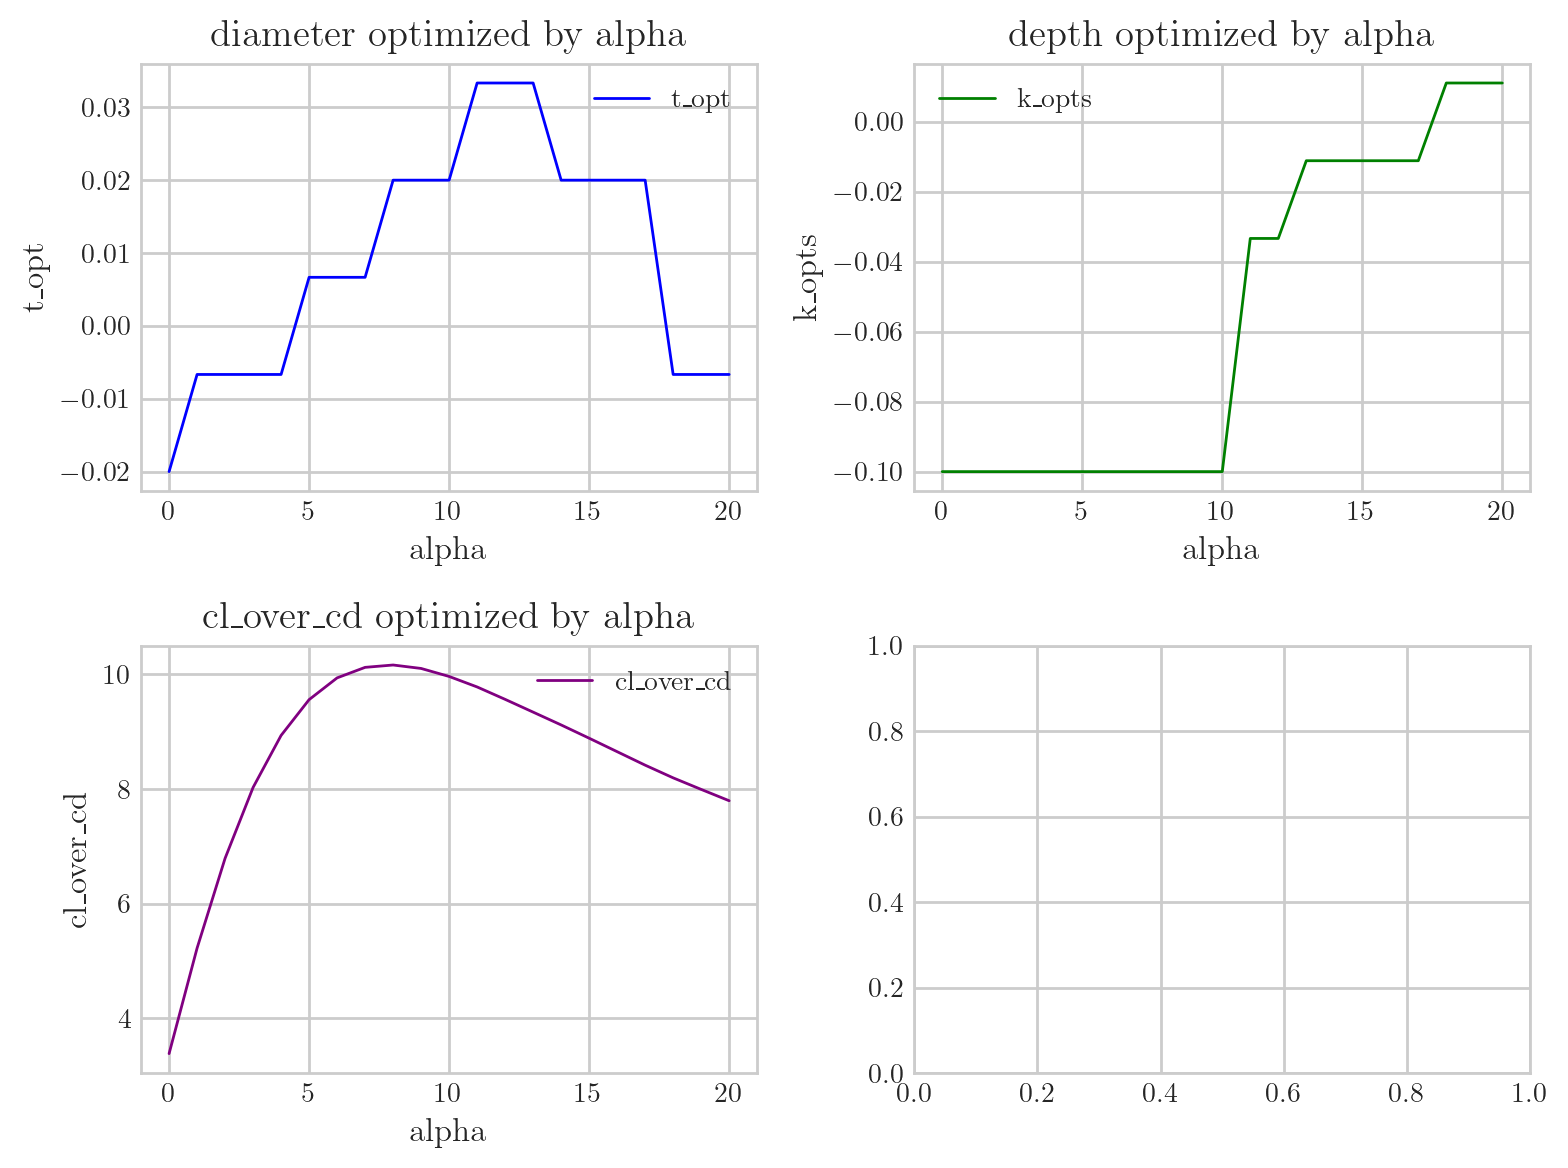
\includegraphics[width=\textwidth]{Pics/résultats pas alpha 3D.png}
        \caption{Tracer de t et k optimaux pour chaque alpha}
        \label{fig:graph}
    \end{minipage}
    \caption{Résultats 3D optimaux (finesse) de diamètre et cambrure par alpha}
    \label{fig:opti alpha 3d}
\end{figure}

\textbf{On observe que le diamètre optimal augmente avec $\alpha$ jusqu'à 13° puis diminue. La cambrure sature à sa valeurs minimale en dessous de 10° puis augumente avec $\alpha$ }

\subsection{3D - résultats moyennes pondérées par Gaussienne}


\begin{figure}[h!]
    \centering
    \subfigure[$\delta diamètre$ selon les paramètres de la Gaussienne]{
        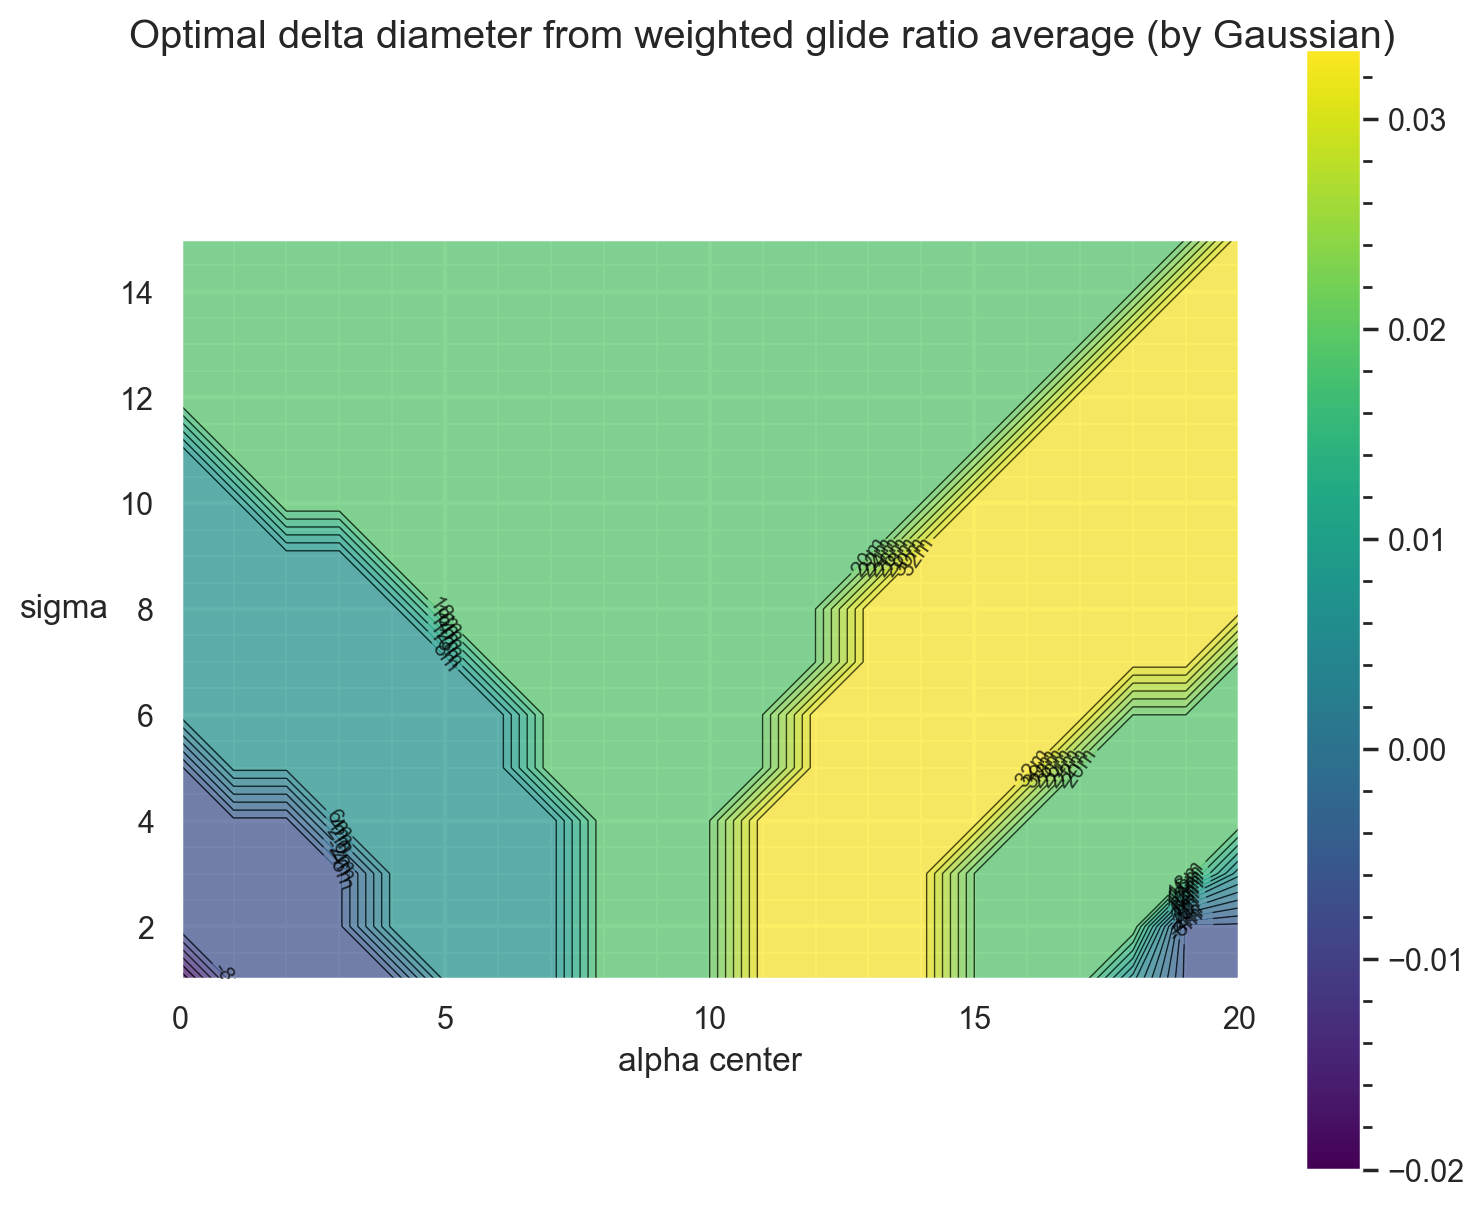
\includegraphics[width=0.45\textwidth]{Pics/diametre gaussian.png}
        \label{fig:diametre gaussien}
    }
    \hfill 
    \subfigure[$\delta cambrure$ selon les paramètres de la Gaussienne]{
        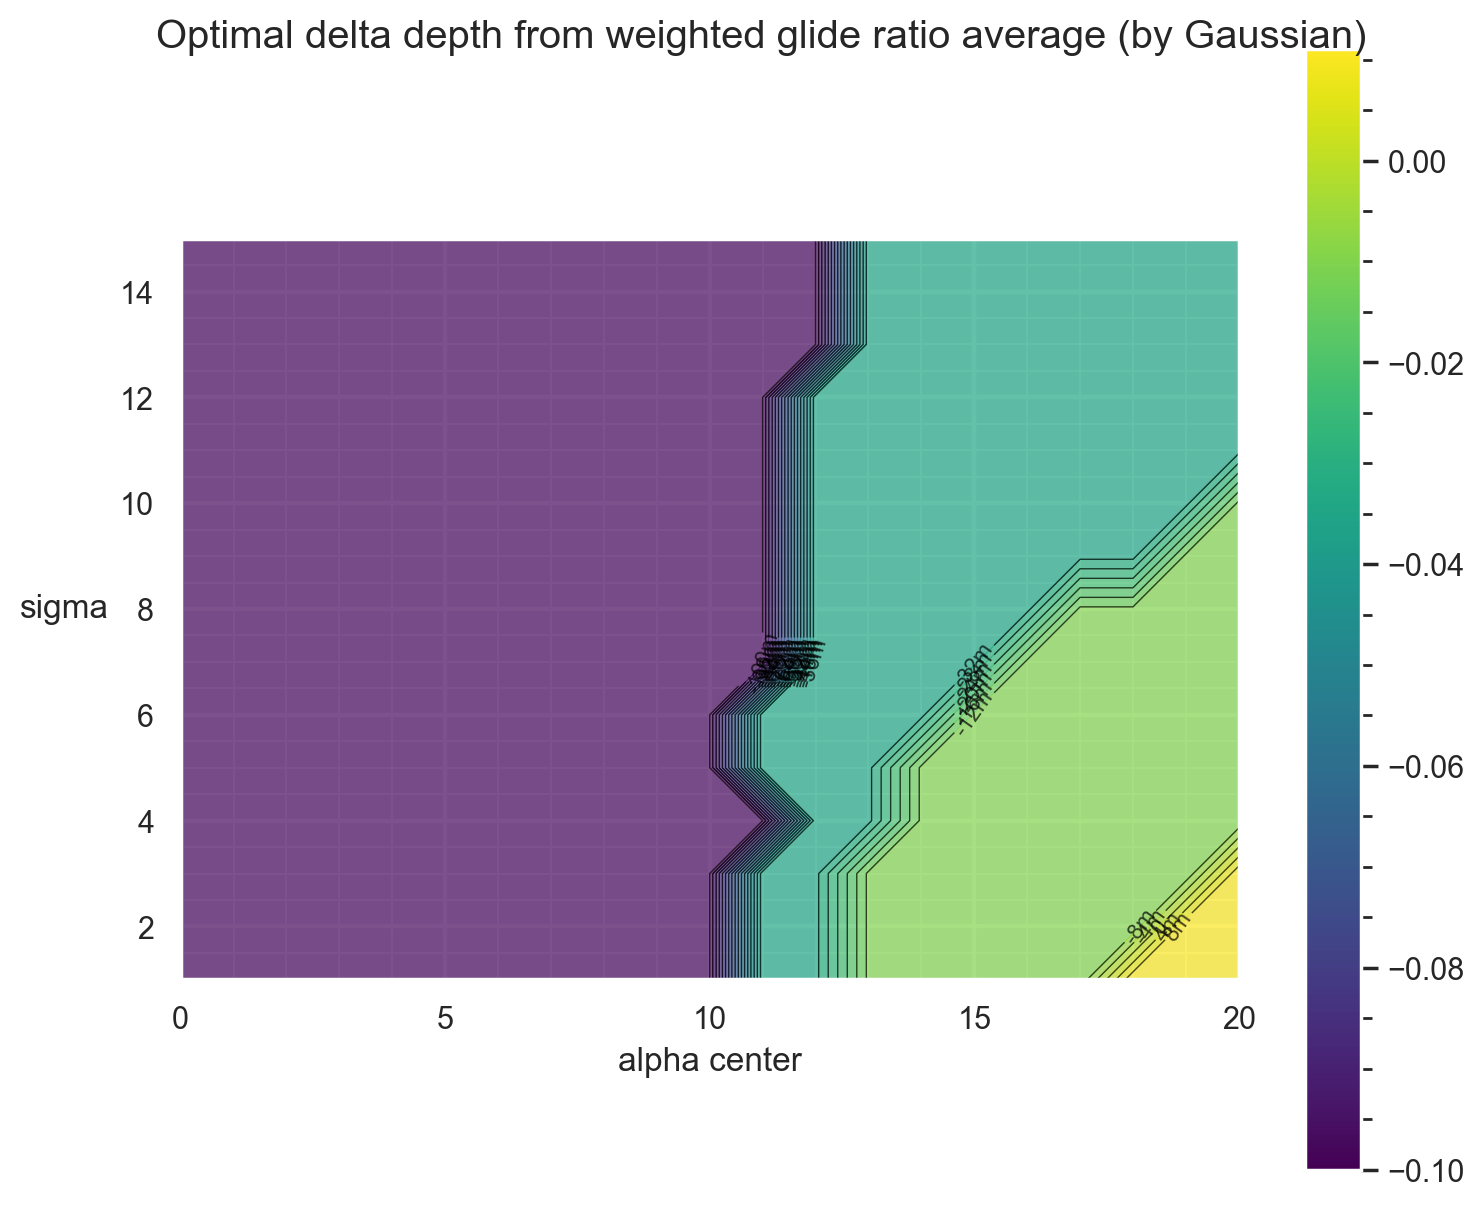
\includegraphics[width=0.45\textwidth]{Pics/depth gaussian.png}
        \label{fig:cambrure gaussien}
    }
    \caption{Sensibilté des résultats 3d en fonction de l'écart-type $\sigma$ et de la valeurs centrale $\alpha_{center}$ de la Gaussienne}
    \label{fig:gaussian sensibility}
\end{figure}

    Sur la figure \ref{fig:gaussian sensibility} (comme sur la figure \ref{fig:gaussian sensibility 2d}), on rappelle que $\sigma$ proche de zéro signife un écart-type quasi nul, i.e. on retrouve les mêmes résultats que sur la figure \ref{fig:opti alpha 3d}. A l'inverse, $\sigma$ grand signifie qu'on augmente l'influence des angles autours de $\alpha_{center}$ sur la moyenne pondérée; fonction objective de l'optimisation. \\

    \textbf{ On observe qu'augmenter $\sigma$ diminue la cambrure optimale. Le comportement est identique pour le diamètre si $\alpha_{center}$ est supérieur à 15°; le comportement inverse en dessous de 15°}
    

\subsection{3D - Exemple de résultat}
Avec une Gaussienne de paramètres \textbf{center = 7° et sigma = 8}, les valeurs qui maximisent la fonction objective (moyenne pondérée de finesse aérodynamique) sont :
\begin{itemize}
    \item $\delta diameter$ : 0.02
    \item $\delta depth$ : -0.1
\end{itemize}
\smallskip

\textbf{Les valeurs de diamètre et cambrure optimaux ainsi obtenus en 3D sont : 
}
\begin{itemize}
    \item t : 0.090 0.086 0.085 0.083 0.081 0.080 0.080  0.080 0.080 0.080 0.080  0.080 0.080 0.080 0.080 0.081 0.083 0.085 0.087 0.090
    \item k : 0.045 0.043 0.043 0.041 0.040 0.040 0.040  0.040 0.040 0.040 0.040 0.040 0.040 0.040  0.040 0.040 0.041 0.043 0.043 0.045
\end{itemize}
\smallskip

\textbf{A comparer avec les valeurs initiales :}
\begin{itemize}
    \item t : 0.07 0.067 0.065 0.063 0.061 0.06 0.06  0.06 0.06 0.06  0.06  0.06 0.06 0.06  0.06 0.061 0.063 0.065 0.067 0.07
    \item k : 0.034 0.05 0.0645 0.0686 0.072 0.075 0.08 0.08 0.08 0.08 0.08 0.08 0.08 0.08 0.075 0.072 0.0686 0.0645 0.05 0.034
\end{itemize}

\textbf{On note donc une tendance (en 3D) à augumenter le diamètre du BA et diminuer la cambrure du kite. }


\section{ Limites et Etudes Complémentaires}

\subsection{Limites}

Tout d'abord Breukels ne prend en compte que le diamètre et la cambrure maximal d'un profil, \textbf{la position de la cambrure maximale d'un profil n'est donc pas prise en compte}. \\

Ensuite, l'étude réalisée \textbf{ne fait pas intervenir de critère de stabilité.} Il sera sujet par suite d'une telle étude avec les résultats obtenus dans ce papier.\\

De plus, le choix de la fonction objective pour la recherche d'un optimum (moyenne pondérée par une Gaussienne) est peu justifiée. Connaître la valeurs d'un angle d'attaque pour lequel on souhaite optimiser une fonction ( finesse, stabilité, portance...) permettrait d'avoir un résultat plus pertinant. \textbf{Mesurer les angles d'attaques principaux lors des essais kite, peut-être avec l'extended Karmann Filter (EKF)} fournit par Kite Power, permettrait de répondre à ce problème. Le choix de sigma et alpha center dans la Gaussienne sont, eux aussi, criticables.\\

Finalement les fonctions d'optimisation d'Aerosandbox ne sont pas applicables à la VSM. Elles sont cependant utilisées pour optimiser la fonction de Breukels (2 paramètres). \\
Aerosandbox peut aussi représenter et optimiser les profils avec 10 paramètres (Kulfan parameters). Ce n'est pas le sujet de ce papier, cependant c'est une façon différente d'aborder le problème. 

\begin{figure}[H]
    \centering
    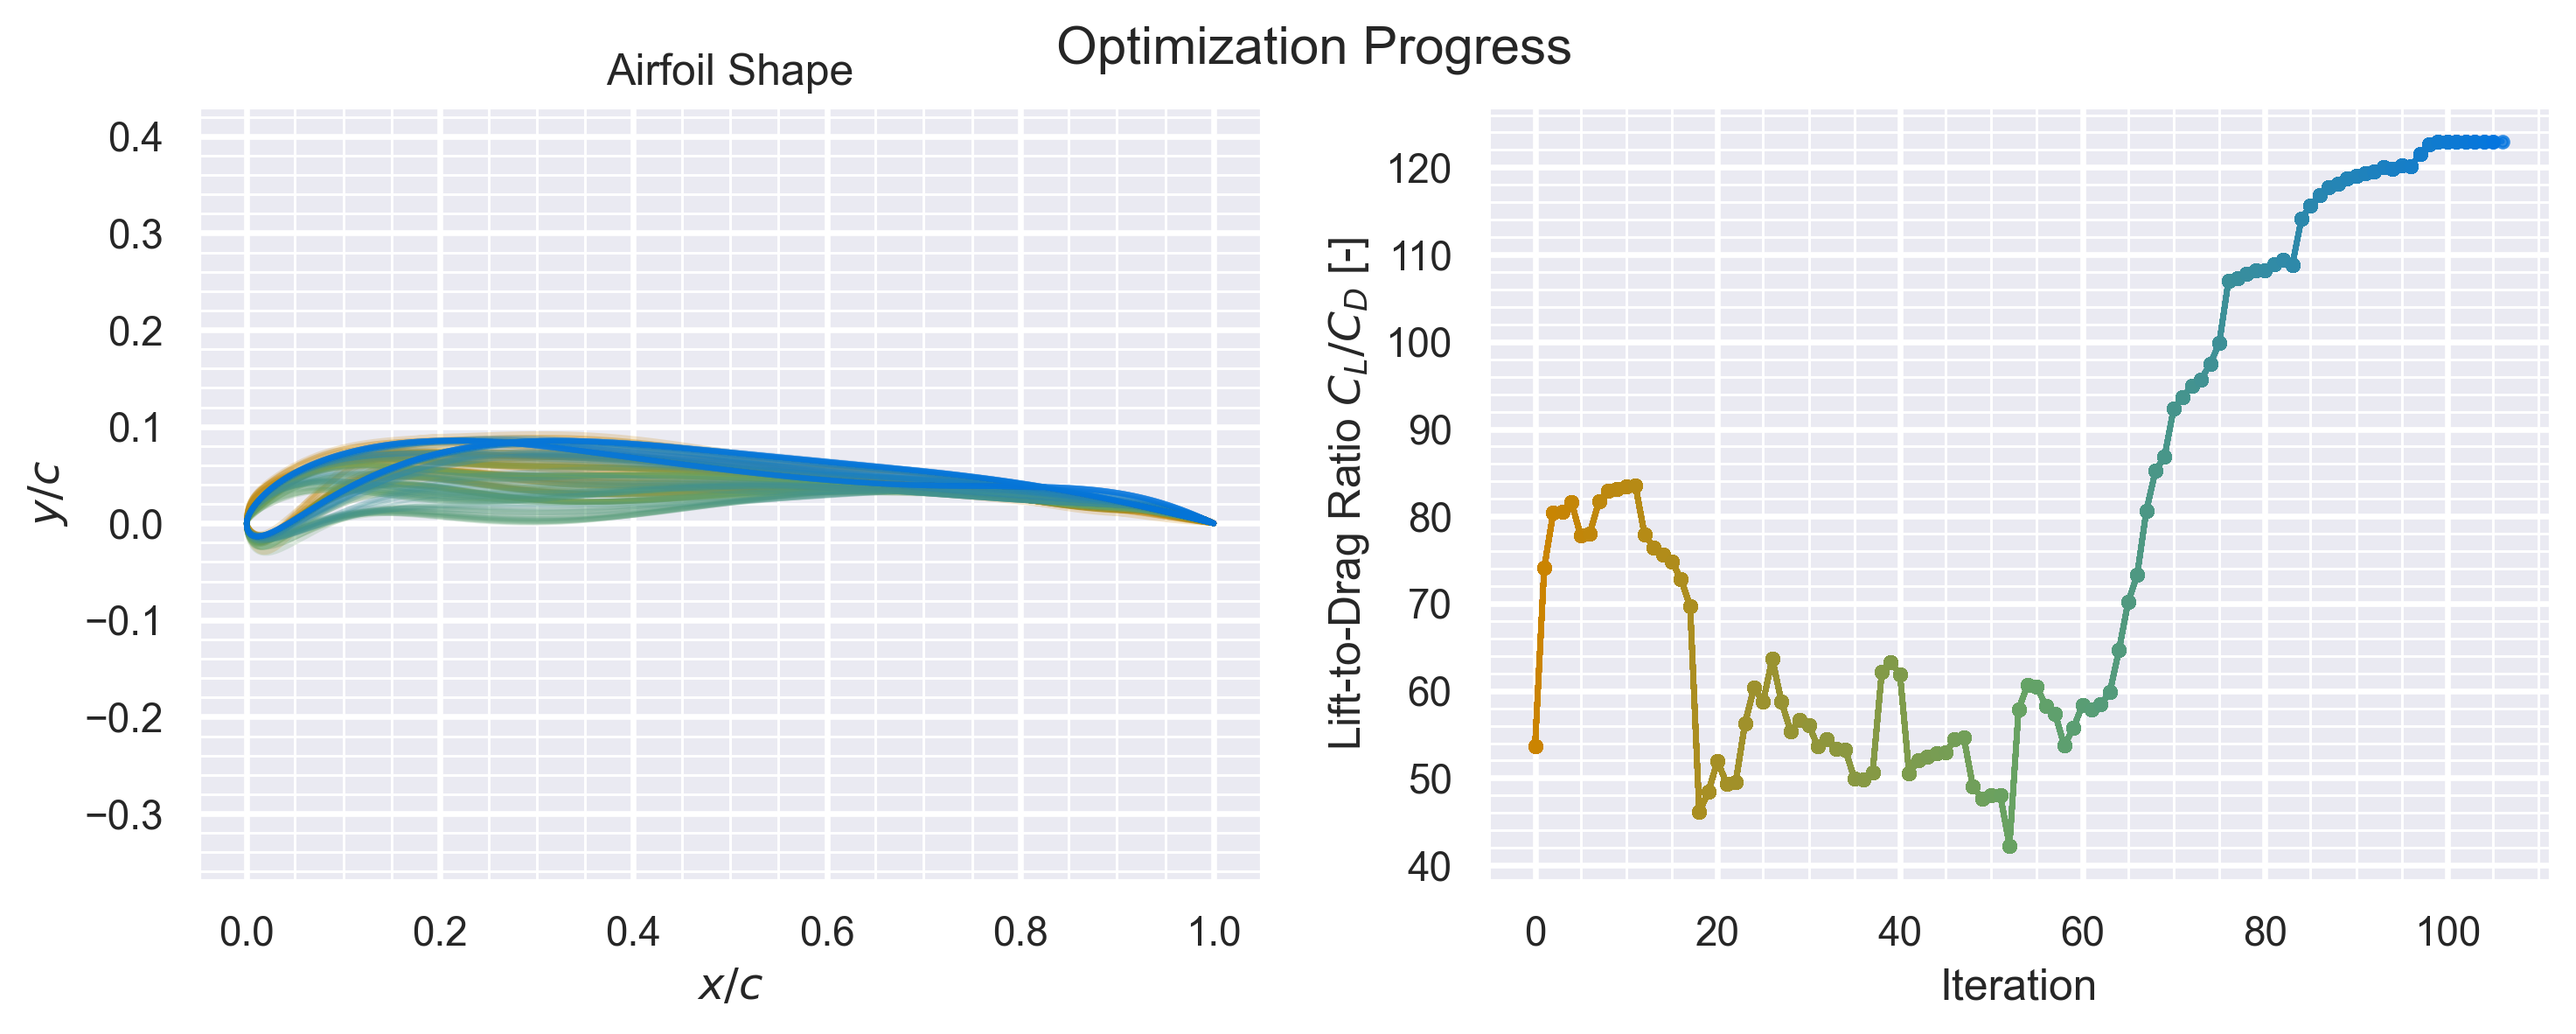
\includegraphics[width=0.5\textwidth]{Pics/optim neuralfoil.png}  
    \caption{Optimisation réalisée avec Aerosandbox sur des profils dis "de Kulfan"}
    \label{fig:kulfan}
\end{figure}

\subsection{Etudes complémentaires}

\begin{itemize}
    \item Comparer sur NeuralFoil et/ou XFoil le profil actuel d’une VG avec le profil optimisé trouvé par OptimXBreukels
    \item Comparer aussi le Cm des 2 profils -> potentiellement conclure sur un profil + performant + stable ?
    \item Créer une base de données d'airfoils polars grâce à Aerosandbox ? qui prend en compte les 3 paramètres (diameter, x depth et depth) et les faire tourner en 2D et ou sur la VSM pour trouver le profil optimal
    \item Faire un chapitre de comparaison des 10m2 classiques vs Hybrid avec profil à caisson, quantifier l'impact de la double peau
\end{itemize}

\end{document}